\section{寄存器描述}
\regover{
{\hyperref[qdec-qdec0-ctrl0]{qdec0\_ctrl0}}&QDEC0 control0
\\
\hline
{\hyperref[qdec-qdec0-ctrl1]{qdec0\_ctrl1}}&QDEC0 control1
\\
\hline
{\hyperref[qdec-qdec0-value]{qdec0\_value}}&QDEC0 value
\\
\hline
{\hyperref[qdec-qdec0-int-en]{qdec0\_int\_en}}&QDEC0 interrupt enable
\\
\hline
{\hyperref[qdec-qdec0-int-sts]{qdec0\_int\_sts}}&QDEC0 interrupt status
\\
\hline
{\hyperref[qdec-qdec0-int-clr]{qdec0\_int\_clr}}&QDEC0 interrupt clear
\\
\hline
{\hyperref[qdec-qdec1-ctrl0]{qdec1\_ctrl0}}&QDEC1 control0
\\
\hline
{\hyperref[qdec-qdec1-ctrl1]{qdec1\_ctrl1}}&QDEC1 control1
\\
\hline
{\hyperref[qdec-qdec1-value]{qdec1\_value}}&QDEC1 value
\\
\hline
{\hyperref[qdec-qdec1-int-en]{qdec1\_int\_en}}&QDEC1 interrupt enable
\\
\hline
{\hyperref[qdec-qdec1-int-sts]{qdec1\_int\_sts}}&QDEC1 interrupt status
\\
\hline
{\hyperref[qdec-qdec1-int-clr]{qdec1\_int\_clr}}&QDEC1 interrupt clear
\\
\hline
{\hyperref[qdec-qdec2-ctrl0]{qdec2\_ctrl0}}&QDEC2 control0
\\
\hline
{\hyperref[qdec-qdec2-ctrl1]{qdec2\_ctrl1}}&QDEC2 control1
\\
\hline
{\hyperref[qdec-qdec2-value]{qdec2\_value}}&QDEC2 value
\\
\hline
{\hyperref[qdec-qdec2-int-en]{qdec2\_int\_en}}&QDEC2 interrupt enable
\\
\hline
{\hyperref[qdec-qdec2-int-sts]{qdec2\_int\_sts}}&QDEC2 interrupt status
\\
\hline
{\hyperref[qdec-qdec2-int-clr]{qdec2\_int\_clr}}&QDEC2 interrupt clear
\\
\hline
}

\subsection{qdec0\_ctrl0}
\label{qdec-qdec0-ctrl0}
地址:0x4000a800
 \begin{figure}[H]
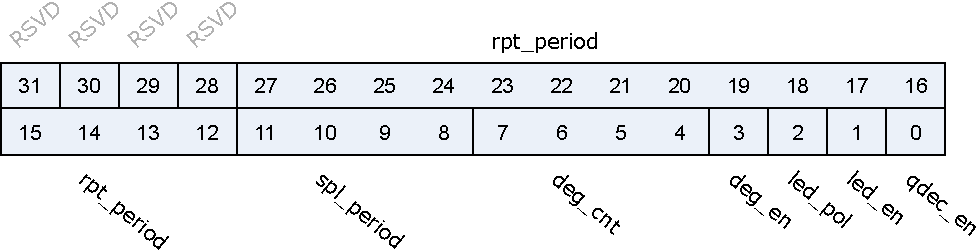
\includegraphics{qdec_qdec0_ctrl0.pdf}
\end{figure}

\regdes{31:28&RSVD& & & \\\hline
27:12&rpt\_period&r/w&16'd10&"RPT" report period in [samples/report]. Specifies the number of samples to be accumulated in the ACC1 register before the RPT\_RDY and DBL\_RDY events can be generated \par "RPT\_US" report period in [us/report] = SP * RP
\\\hline
11:8&spl\_period&r/w&4'h2&"SPL" sample period in [us/sample]. The SAMPLE register will be updated for every new sample \par 0:  32 us \par 1:  64 \par 2: 128 \par 3: 256 \par 4: 512 \par 5:   1 ms \par 6:   2 \par 7:   4 \par 8:   8 \par 9:  16 \par A:  32 \par B:  65 \par C: 131
\\\hline
7:4&deg\_cnt&r/w&0&\\\hline
3&deg\_en&r/w&0&deglitch\\\hline
2&led\_pol&r/w&1&led polarity\\\hline
1&led\_en&r/w&0&\\\hline
0&qdec\_en&r/w&0&\\\hline

}
\subsection{qdec0\_ctrl1}
\label{qdec-qdec0-ctrl1}
地址:0x4000a804
 \begin{figure}[H]
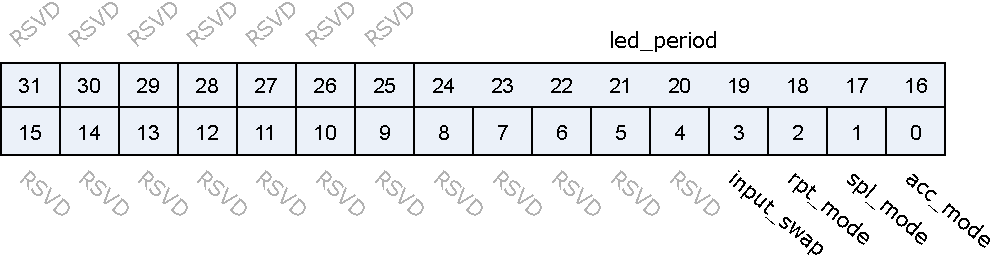
\includegraphics{qdec_qdec0_ctrl1.pdf}
\end{figure}

\regdes{31:25&RSVD& & & \\\hline
24:16&led\_period&r/w&0&Period in us the LED is switched on prior to sampling\\\hline
15:4&RSVD& & & \\\hline
3&input\_swap&r/w&0&input a/b swap\\\hline
2&rpt\_mode&r/w&0&rpt option  0: Count time only if sample change  1: Continue time\\\hline
1&spl\_mode&r/w&0&spl option  0: Stop sample if rpt\_rdy  1: Continue sample\\\hline
0&acc\_mode&r/w&1&acc option  0: Stop accumulate if overflow  1: Continue accumulate\\\hline

}
\subsection{qdec0\_value}
\label{qdec-qdec0-value}
地址:0x4000a808
 \begin{figure}[H]
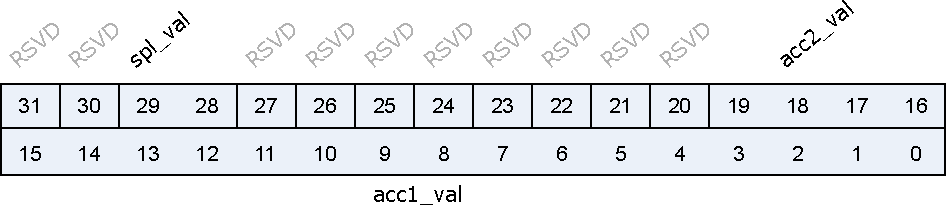
\includegraphics{qdec_qdec0_value.pdf}
\end{figure}

\regdes{31:30&RSVD& & & \\\hline
29:28&spl\_val&r&0&Sample value. Direction of last change \par 00: no change \par 01: clockwise \par 11: counter-clockwise \par 10: Error
\\\hline
27:20&RSVD& & & \\\hline
19:16&acc2\_val&r&0&Double error accumulation (0~15)\\\hline
15:0&acc1\_val&r&0&Sample accumulation (-1024~1023)\\\hline

}
\subsection{qdec0\_int\_en}
\label{qdec-qdec0-int-en}
地址:0x4000a810
 \begin{figure}[H]
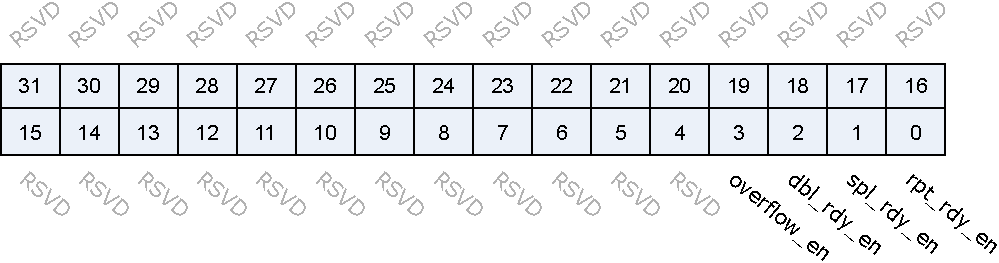
\includegraphics{qdec_qdec0_int_en.pdf}
\end{figure}

\regdes{31:4&RSVD& & & \\\hline
3&overflow\_en&r/w&0&\\\hline
2&dbl\_rdy\_en&r/w&0&\\\hline
1&spl\_rdy\_en&r/w&0&\\\hline
0&rpt\_rdy\_en&r/w&1&\\\hline

}
\subsection{qdec0\_int\_sts}
\label{qdec-qdec0-int-sts}
地址:0x4000a814
 \begin{figure}[H]
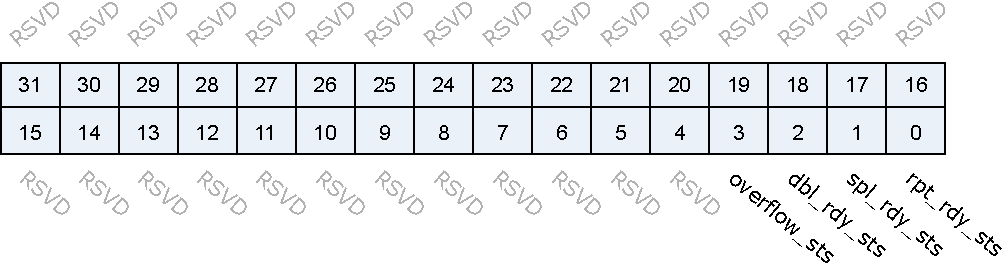
\includegraphics{qdec_qdec0_int_sts.pdf}
\end{figure}

\regdes{31:4&RSVD& & & \\\hline
3&overflow\_sts&r&0&ACC1 or ACC2 overflow\\\hline
2&dbl\_rdy\_sts&r&0&ACC2 double error\\\hline
1&spl\_rdy\_sts&r&0&Event being generated for every new sample value written to the SAMPLE register\\\hline
0&rpt\_rdy\_sts&r&0&Non-null report ready\\\hline

}
\subsection{qdec0\_int\_clr}
\label{qdec-qdec0-int-clr}
地址:0x4000a818
 \begin{figure}[H]
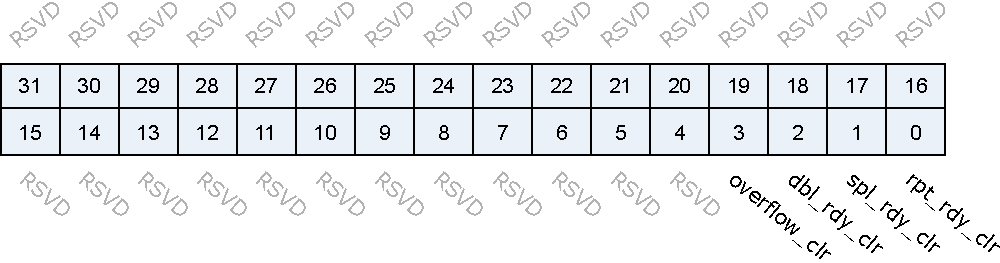
\includegraphics{qdec_qdec0_int_clr.pdf}
\end{figure}

\regdes{31:4&RSVD& & & \\\hline
3&overflow\_clr&w1c&0&\\\hline
2&dbl\_rdy\_clr&w1c&0&\\\hline
1&spl\_rdy\_clr&w1c&0&\\\hline
0&rpt\_rdy\_clr&w1c&0&\\\hline

}
\subsection{qdec1\_ctrl0}
\label{qdec-qdec1-ctrl0}
地址:0x4000a840
 \begin{figure}[H]
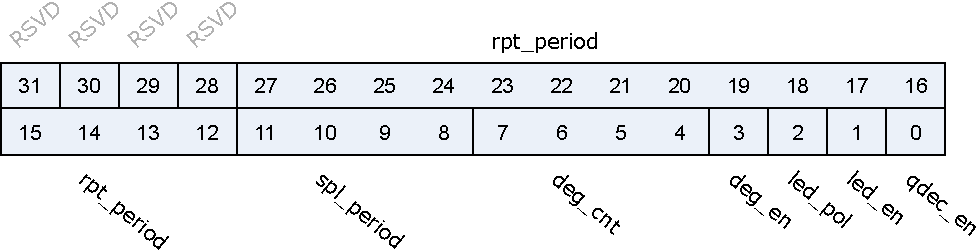
\includegraphics{qdec_qdec1_ctrl0.pdf}
\end{figure}

\regdes{31:28&RSVD& & & \\\hline
27:12&rpt\_period&r/w&16'd10&"RPT" report period in [samples/report]. Specifies the number of samples to be accumulated in the ACC1 register before the RPT\_RDY and DBL\_RDY events can be generated \par "RPT\_US" report period in [us/report] = SP * RP
\\\hline
11:8&spl\_period&r/w&4'h2&"SPL" sample period in [us/sample]. The SAMPLE register will be updated for every new sample \par 0:  32 us \par 1:  64 \par 2: 128 \par 3: 256 \par 4: 512 \par 5:   1 ms \par 6:   2 \par 7:   4 \par 8:   8 \par 9:  16 \par A:  32 \par B:  65 \par C: 131
\\\hline
7:4&deg\_cnt&r/w&0&\\\hline
3&deg\_en&r/w&0&deglitch\\\hline
2&led\_pol&r/w&1&led polarity\\\hline
1&led\_en&r/w&0&\\\hline
0&qdec\_en&r/w&0&\\\hline

}
\subsection{qdec1\_ctrl1}
\label{qdec-qdec1-ctrl1}
地址:0x4000a844
 \begin{figure}[H]
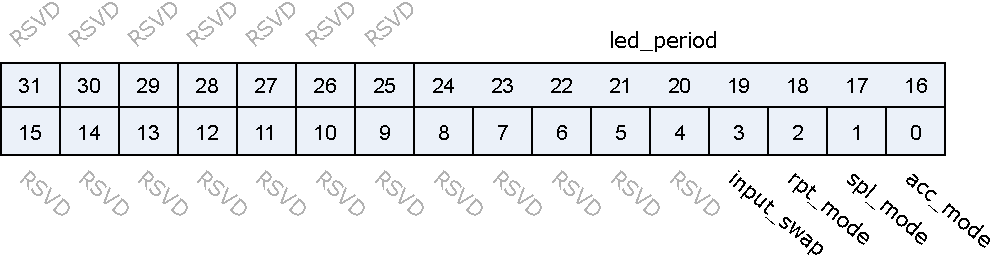
\includegraphics{qdec_qdec1_ctrl1.pdf}
\end{figure}

\regdes{31:25&RSVD& & & \\\hline
24:16&led\_period&r/w&0&Period in us the LED is switched on prior to sampling\\\hline
15:4&RSVD& & & \\\hline
3&input\_swap&r/w&0&input a/b swap\\\hline
2&rpt\_mode&r/w&0&rpt option  0: Count time only if sample change  1: Continue time\\\hline
1&spl\_mode&r/w&0&spl option  0: Stop sample if rpt\_rdy  1: Continue sample\\\hline
0&acc\_mode&r/w&1&acc option  0: Stop accumulate if overflow  1: Continue accumulate\\\hline

}
\subsection{qdec1\_value}
\label{qdec-qdec1-value}
地址:0x4000a848
 \begin{figure}[H]
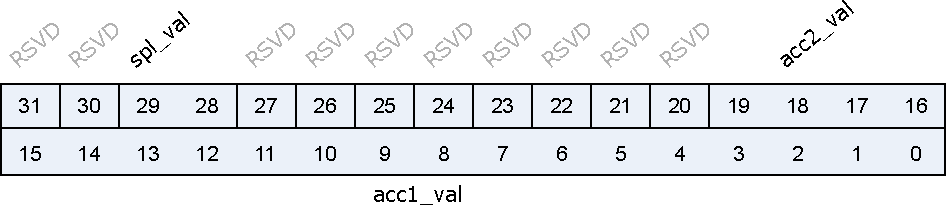
\includegraphics{qdec_qdec1_value.pdf}
\end{figure}

\regdes{31:30&RSVD& & & \\\hline
29:28&spl\_val&r&0&Sample value. Direction of last change \par 00: no change \par 01: clockwise \par 11: counter-clockwise \par 10: Error
\\\hline
27:20&RSVD& & & \\\hline
19:16&acc2\_val&r&0&Double error accumulation (0~15)\\\hline
15:0&acc1\_val&r&0&Sample accumulation (-1024~1023)\\\hline

}
\subsection{qdec1\_int\_en}
\label{qdec-qdec1-int-en}
地址:0x4000a850
 \begin{figure}[H]
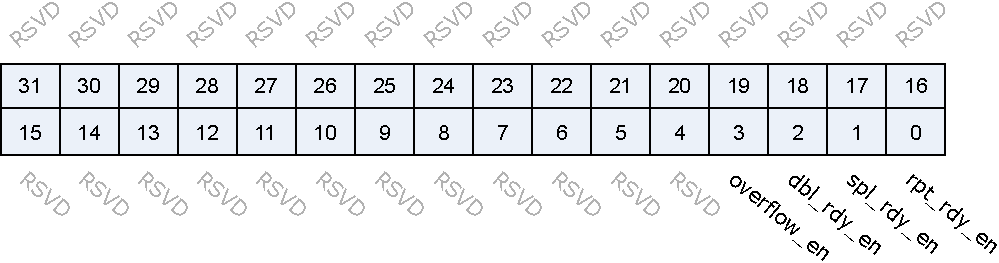
\includegraphics{qdec_qdec1_int_en.pdf}
\end{figure}

\regdes{31:4&RSVD& & & \\\hline
3&overflow\_en&r/w&0&\\\hline
2&dbl\_rdy\_en&r/w&0&\\\hline
1&spl\_rdy\_en&r/w&0&\\\hline
0&rpt\_rdy\_en&r/w&1&\\\hline

}
\subsection{qdec1\_int\_sts}
\label{qdec-qdec1-int-sts}
地址:0x4000a854
 \begin{figure}[H]
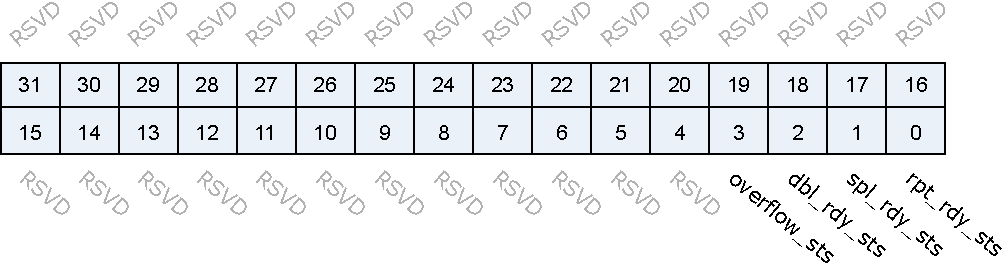
\includegraphics{qdec_qdec1_int_sts.pdf}
\end{figure}

\regdes{31:4&RSVD& & & \\\hline
3&overflow\_sts&r&0&ACC1 or ACC2 overflow\\\hline
2&dbl\_rdy\_sts&r&0&ACC2 double error\\\hline
1&spl\_rdy\_sts&r&0&Event being generated for every new sample value written to the SAMPLE register\\\hline
0&rpt\_rdy\_sts&r&0&Non-null report ready\\\hline

}
\subsection{qdec1\_int\_clr}
\label{qdec-qdec1-int-clr}
地址:0x4000a858
 \begin{figure}[H]
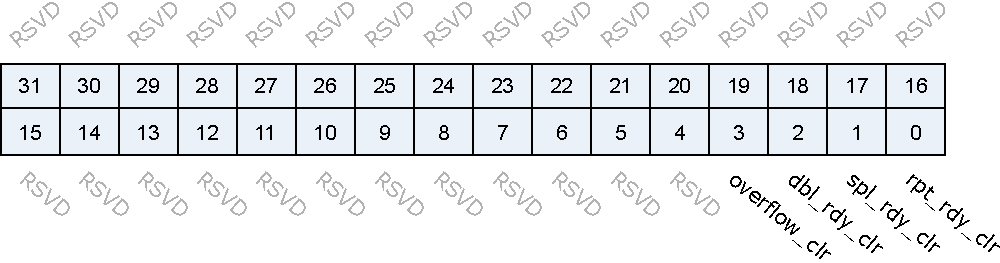
\includegraphics{qdec_qdec1_int_clr.pdf}
\end{figure}

\regdes{31:4&RSVD& & & \\\hline
3&overflow\_clr&w1c&0&\\\hline
2&dbl\_rdy\_clr&w1c&0&\\\hline
1&spl\_rdy\_clr&w1c&0&\\\hline
0&rpt\_rdy\_clr&w1c&0&\\\hline

}
\subsection{qdec2\_ctrl0}
\label{qdec-qdec2-ctrl0}
地址:0x4000a880
 \begin{figure}[H]
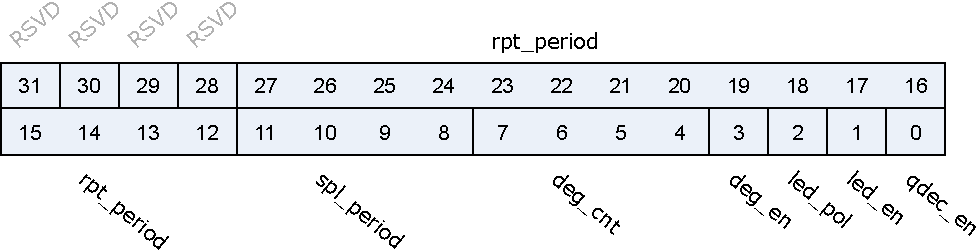
\includegraphics{qdec_qdec2_ctrl0.pdf}
\end{figure}

\regdes{31:28&RSVD& & & \\\hline
27:12&rpt\_period&r/w&16'd10&"RPT" report period in [samples/report]. Specifies the number of samples to be accumulated in the ACC1 register before the RPT\_RDY and DBL\_RDY events can be generated \par "RPT\_US" report period in [us/report] = SP * RP
\\\hline
11:8&spl\_period&r/w&4'h2&"SPL" sample period in [us/sample]. The SAMPLE register will be updated for every new sample \par 0:  32 us \par 1:  64 \par 2: 128 \par 3: 256 \par 4: 512 \par 5:   1 ms \par 6:   2 \par 7:   4 \par 8:   8 \par 9:  16 \par A:  32 \par B:  65 \par C: 131
\\\hline
7:4&deg\_cnt&r/w&0&\\\hline
3&deg\_en&r/w&0&deglitch\\\hline
2&led\_pol&r/w&1&led polarity\\\hline
1&led\_en&r/w&0&\\\hline
0&qdec\_en&r/w&0&\\\hline

}
\subsection{qdec2\_ctrl1}
\label{qdec-qdec2-ctrl1}
地址:0x4000a884
 \begin{figure}[H]
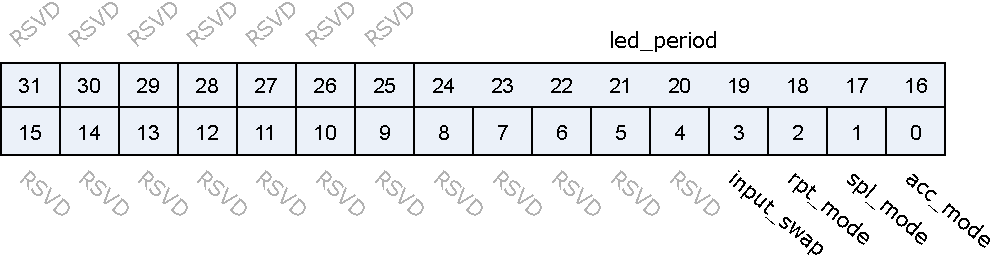
\includegraphics{qdec_qdec2_ctrl1.pdf}
\end{figure}

\regdes{31:25&RSVD& & & \\\hline
24:16&led\_period&r/w&0&Period in us the LED is switched on prior to sampling\\\hline
15:4&RSVD& & & \\\hline
3&input\_swap&r/w&0&input a/b swap\\\hline
2&rpt\_mode&r/w&0&rpt option  0: Count time only if sample change  1: Continue time\\\hline
1&spl\_mode&r/w&0&spl option  0: Stop sample if rpt\_rdy  1: Continue sample\\\hline
0&acc\_mode&r/w&1&acc option  0: Stop accumulate if overflow  1: Continue accumulate\\\hline

}
\subsection{qdec2\_value}
\label{qdec-qdec2-value}
地址:0x4000a888
 \begin{figure}[H]
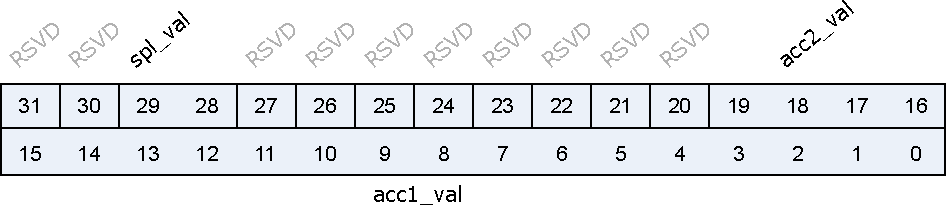
\includegraphics{qdec_qdec2_value.pdf}
\end{figure}

\regdes{31:30&RSVD& & & \\\hline
29:28&spl\_val&r&0&Sample value. Direction of last change \par 00: no change \par 01: clockwise \par 11: counter-clockwise \par 10: Error
\\\hline
27:20&RSVD& & & \\\hline
19:16&acc2\_val&r&0&Double error accumulation (0~15)\\\hline
15:0&acc1\_val&r&0&Sample accumulation (-1024~1023)\\\hline

}
\subsection{qdec2\_int\_en}
\label{qdec-qdec2-int-en}
地址:0x4000a890
 \begin{figure}[H]
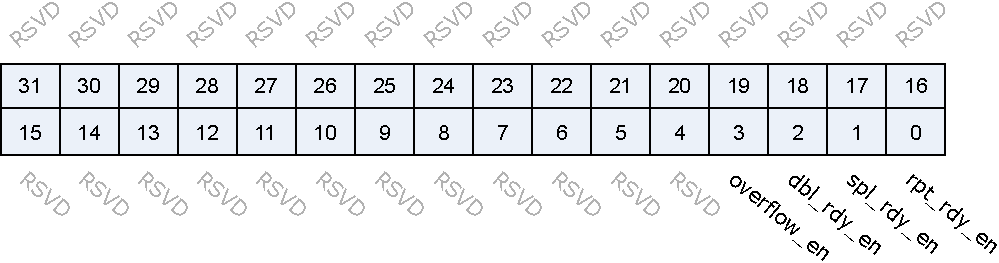
\includegraphics{qdec_qdec2_int_en.pdf}
\end{figure}

\regdes{31:4&RSVD& & & \\\hline
3&overflow\_en&r/w&0&\\\hline
2&dbl\_rdy\_en&r/w&0&\\\hline
1&spl\_rdy\_en&r/w&0&\\\hline
0&rpt\_rdy\_en&r/w&1&\\\hline

}
\subsection{qdec2\_int\_sts}
\label{qdec-qdec2-int-sts}
地址:0x4000a894
 \begin{figure}[H]
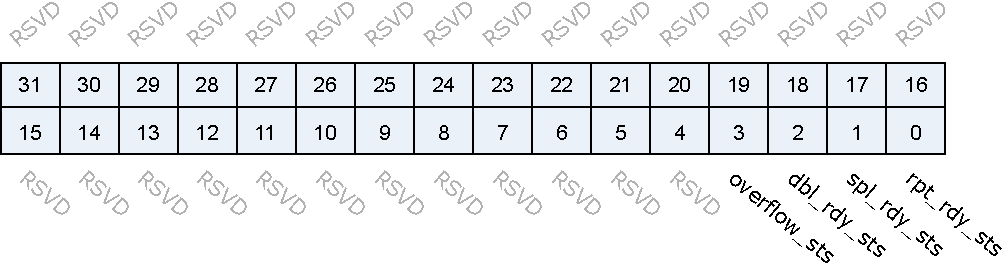
\includegraphics{qdec_qdec2_int_sts.pdf}
\end{figure}

\regdes{31:4&RSVD& & & \\\hline
3&overflow\_sts&r&0&ACC1 or ACC2 overflow\\\hline
2&dbl\_rdy\_sts&r&0&ACC2 double error\\\hline
1&spl\_rdy\_sts&r&0&Event being generated for every new sample value written to the SAMPLE register\\\hline
0&rpt\_rdy\_sts&r&0&Non-null report ready\\\hline

}
\subsection{qdec2\_int\_clr}
\label{qdec-qdec2-int-clr}
地址:0x4000a898
 \begin{figure}[H]
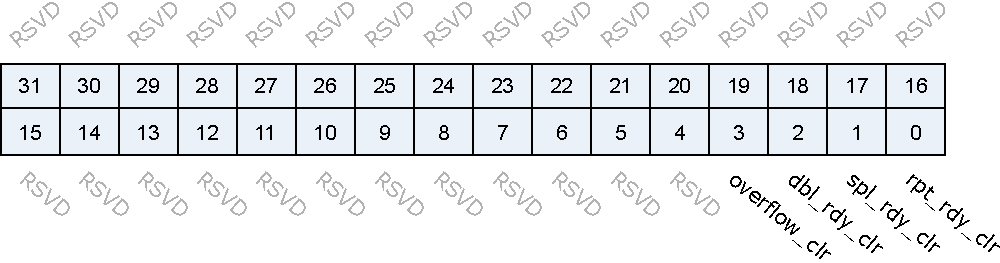
\includegraphics{qdec_qdec2_int_clr.pdf}
\end{figure}

\regdes{31:4&RSVD& & & \\\hline
3&overflow\_clr&w1c&0&\\\hline
2&dbl\_rdy\_clr&w1c&0&\\\hline
1&spl\_rdy\_clr&w1c&0&\\\hline
0&rpt\_rdy\_clr&w1c&0&\\\hline

}
